\newsection
\subsection{BP 1:
  Single wave on a simple beach (Analytic)}

{\bf Documentation:}  PMEL-135, pp 5 \&
18-30.\cite{SynolakisBernard:pmel135}

\subsubsection{Problems encountered}

\begin{itemize}
\item Numerics for analytical solution to wave equation were hard to determine and should be provided in excel file in description of problem. Analytical solution was obtained from problem champion.
\item No analytical solution given for time $t = 25s$
\item Clawpack code does not include maximum runup calculation. Additional module needed to be written. 
\end{itemize}

\subsubsection{What we did}

\begin{itemize}
\item Used $g=1$ and no friction.
\item The bathymetry consists of a deep plateau of constant depth $d$
connected to a sloping beach of angle $\beta = \text{arccot}(19.85)$. 
Note that the toe of the beach is located at $x = X_0 = d \text{cot} \beta$
\item The initial waveform of the wave is given by 
\begin{equation}
\eta(x,0) = H \text{sech}^2(\gamma (x - X_1)/d)
\end{equation}
where $L = \text{arccosh}(\sqrt(20))/\gamma$, $X_1 = X_0 + L$, 
and $\gamma = \sqrt(3H/4d)$. The speed of the wave is given by the following: 
\begin{equation}
u(x,0)=-\sqrt{g/d}\eta(x,0)
\end{equation}
\item Problem was solved on $800\times 2$ grid, where the x domain spanned from -10 to 60.
\item Variable time stepping was allowed based on a CFL number of 0.9
\end{itemize} 

\subsubsection{Gauge comparisons}
Compare the numerically and analytically computer water level dynamics at locations $x/d = 0.25$ and $x/d = 9.95$ during the propagation and reflection of the wave


See \Fig{bp1gauges}.

\begin{figure}[ht]
%\hfil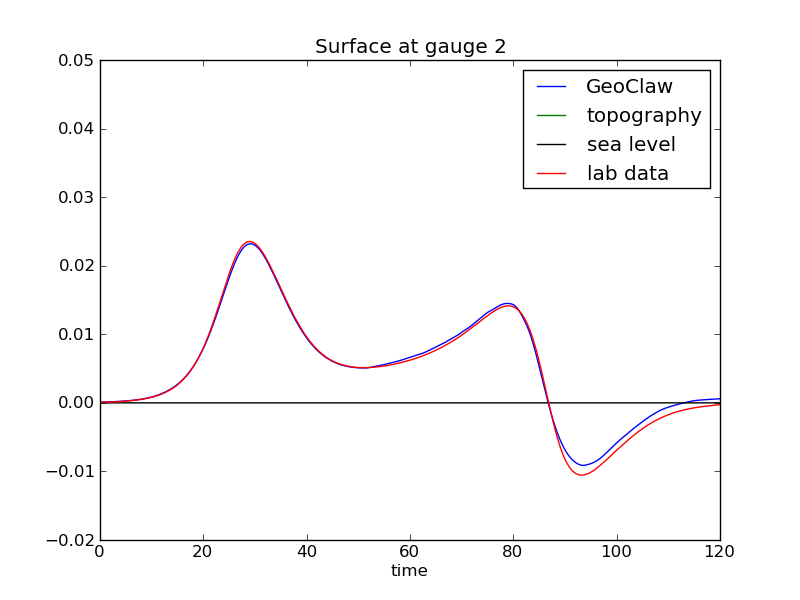
\includegraphics[width=2.8in]{bp1/gauge0002fig300.png}\hfil
%\hfil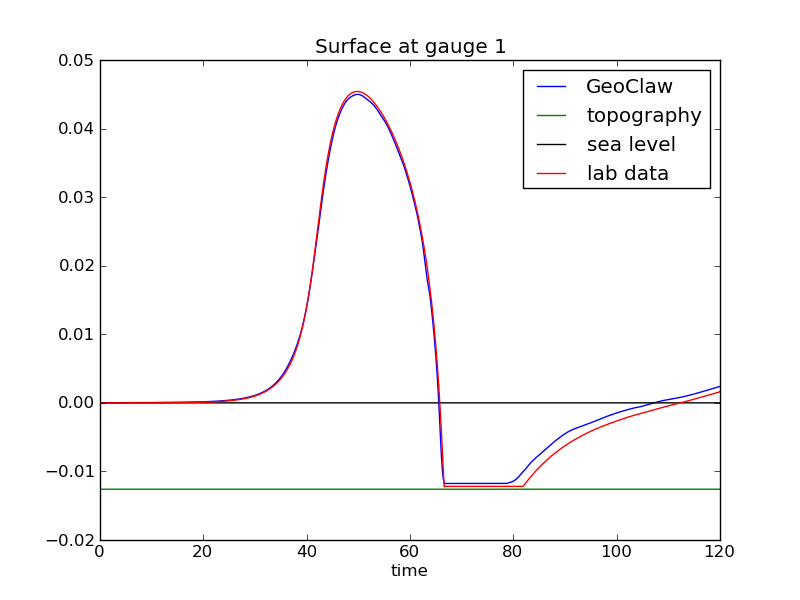
\includegraphics[width=2.8in]{bp1/gauge0001fig300.png}\hfil
\hfil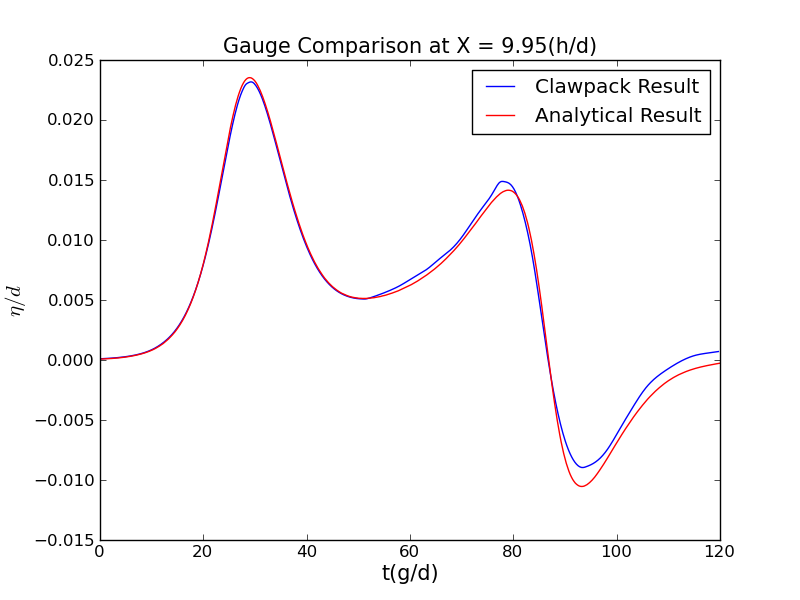
\includegraphics[width=2.8in]{bp1/plotgauge2.png}\hfil
\hfil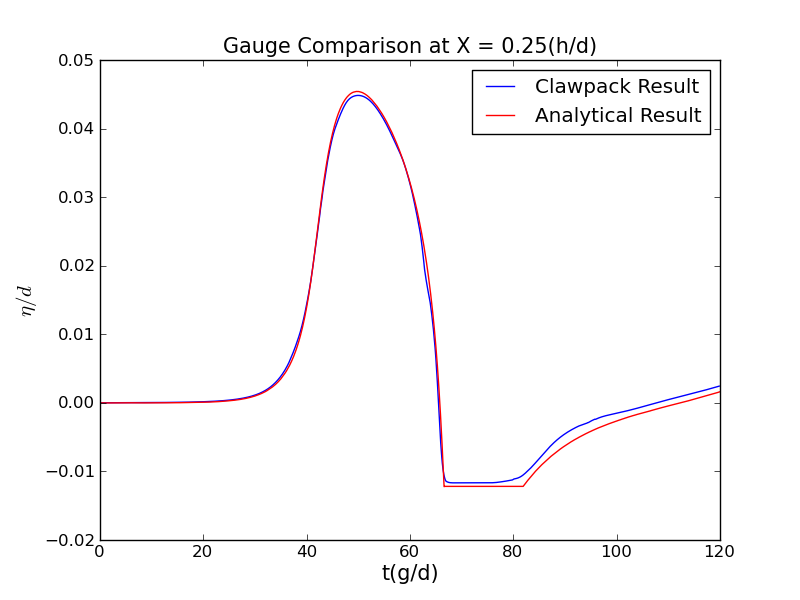
\includegraphics[width=2.8in]{bp1/plotgauge1.png}\hfil
\caption{\label{fig:bp1gauges} 
Left column: Gauge profile at location $x/d = 9.95$.
Right column: Gauge profile at location $x/d = 0.25$.
 }
\end{figure}



\subsubsection{Frame comparisons}
We were asked to
compare the numerically and analytically computed water level profiles at $t = 25(d/g)^{1/2}$, $t = 35(d/g)^{1/2}$, $t = 45(d/g)^{1/2}$, $t = 55(d/g)^{1/2}$, $t = 65(d/g)^{1/2}$.
However, the data file {\tt canonical\_profiles.txt} is missing data for
$t=25(d/g)^{1/2}$ and so we omitted this time.
See \Fig{bp1frames} for the computed and analytic results for the other
times.

\begin{figure}[ht]
\hfil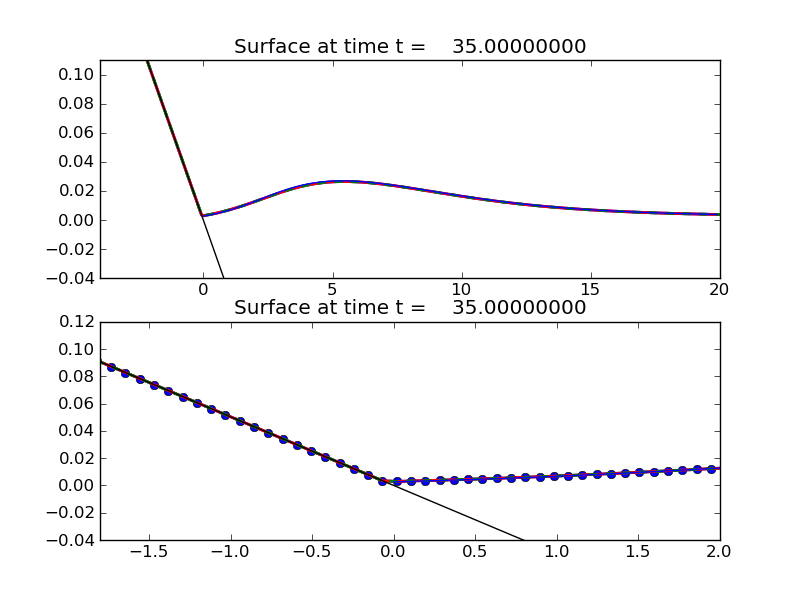
\includegraphics[width=2.8in]{bp1/frame0001fig2.png}\hfil
\hfil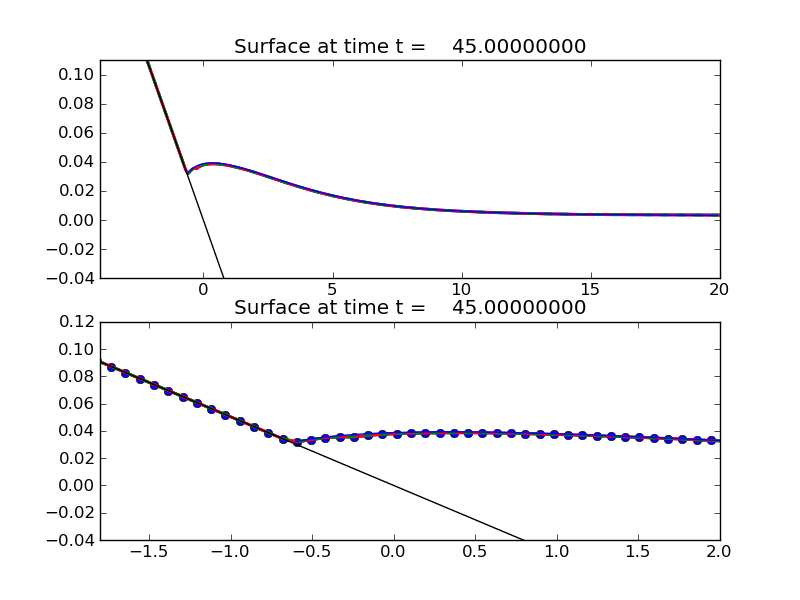
\includegraphics[width=2.8in]{bp1/frame0003fig2.png}\hfil
\vskip 5pt
\hfil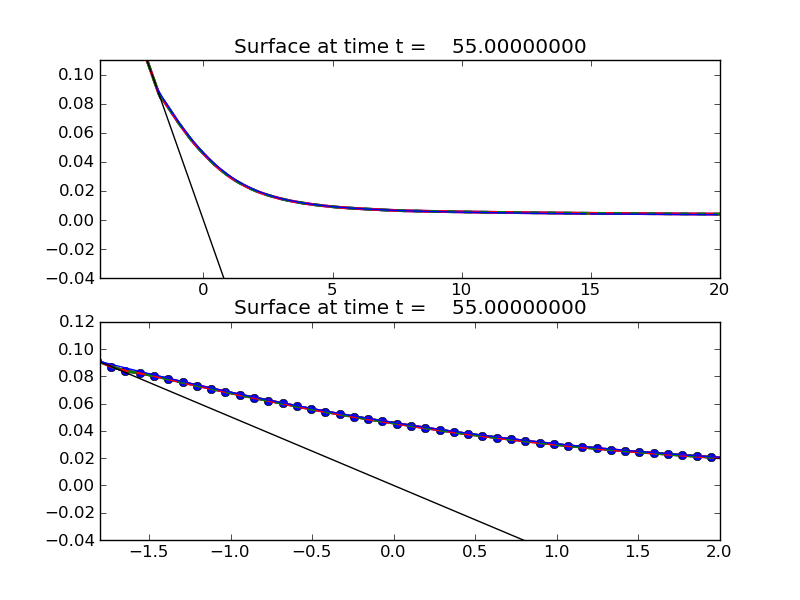
\includegraphics[width=2.8in]{bp1/frame0005fig2.png}\hfil
\hfil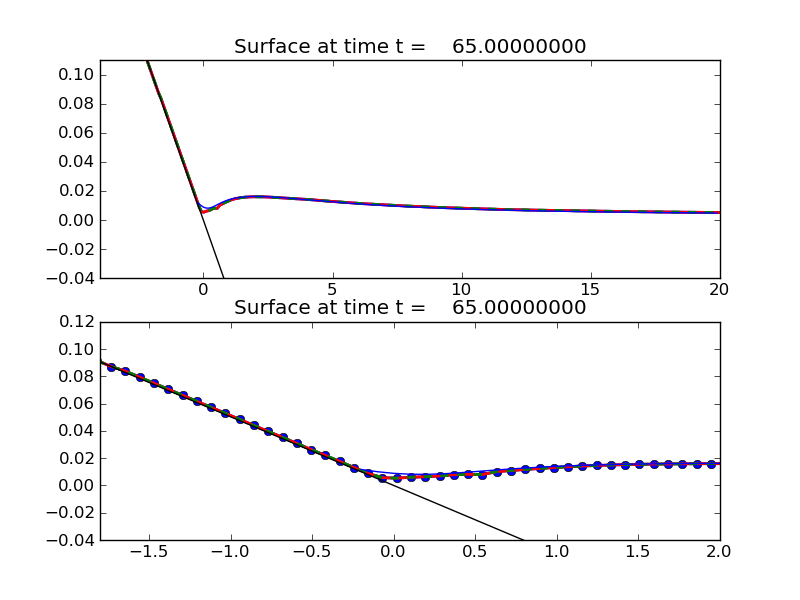
\includegraphics[width=2.8in]{bp1/frame0007fig2.png}\hfil
\caption{\label{fig:bp1frames} 
Frames of solution. Top frame: Full view of incoming wave. Bottom Frame: Zoomed
view of inundation area. The analytic and GeoClaw solutions are both
plotted, but mostly lie on top of one another.}
\end{figure}

\subsection{Maximum Runup}
Compute the maximum runup.
See \Fig{bp1runup}
\begin{figure}[ht]
\hfil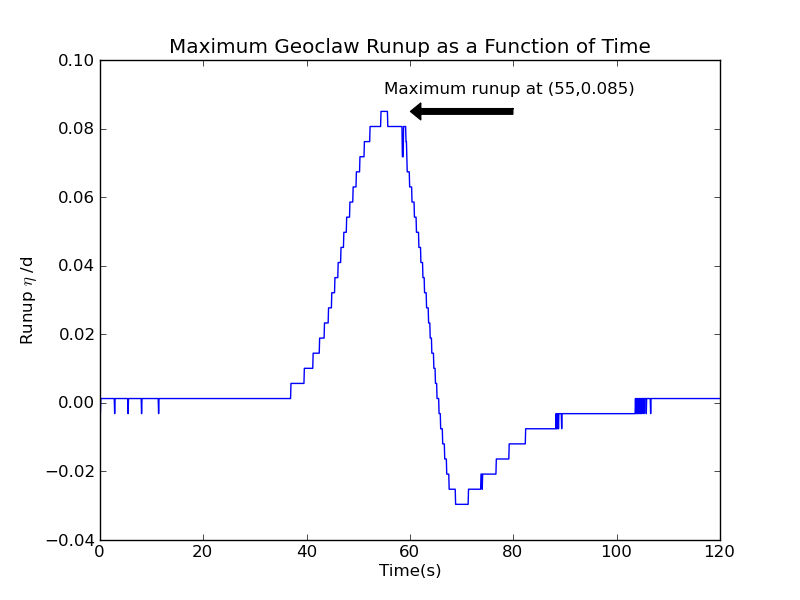
\includegraphics[width=5.5in]{bp1/runup.png}\hfil
\caption{\label{fig:bp1runup} 
Runup on canonical beach as a function of time}
\end{figure}

\subsubsection{Lessons learned}

This is a very relevent benchmark problem because it is a good
application of the shallow water wave equations with an analytic solution
in one dimesion. Because the analytical solution is so complex, an accurate
numerical approximation needs to be provided on the benchmark problem
website to ensure all participants are solving the same problem.
